\subsection{Progettazione architetturale}
Questa fase comincia subito dopo la presentazione e finisce con la data di consegna per la \textit{Revisione di Progettazione}, ovvero \textit{dal 18-01-2021 al 01-03-2021}.\\
In questo periodo verrà individuata una soluzione architetturale che funga da sostegno per l'implementazione del prodotto. Deve soddisfare tutti i requisiti richiesti, oltre ad essere facilmente comprensibile ed attuabile. 

\subsubsection{Progettazione della technology baseline}

Il periodo di progettazione della technology baseline ha inizio il giorno 25-01-2021, successivamente alla revisione dei requisiti, con termine fissato per il giorno 08-02-2021. \\ A causa della concomitanza con la sessione accademica, il team ha fissato la prima \glo{milestone} al termine di questo periodo. Alla scadenza, il gruppo dovrà aver iniziato lo studio delle tecnologie per la \textit{Technology baseline}, oltre ad aver controllato buona parte della documentazione.

\begin{itemize}
\item \textbf{Incremento e verifica dei documenti}: se fosse necessario, i documenti prodotti dal team verranno integrati.

 \item \glo{\textbf{Technology baseline}}: viene fatta un'analisi ad alto livello per comprendere le tecnologie coinvolte, in due passi distinti:
\begin{itemize}
 \item \textbf{Decomposizione del prodotto} in parti, in modo da essere realizzato con risorse sostenibili e costi compatibili;
 \item \textbf{Analisi delle componenti individuate}, in modo da determinare come ciascuna interagisce con le altre.  
 
\end{itemize}
\end{itemize}

\subsubsection{Progettazione e codifica del Proof of Concept}
L'architettura verrà progettata sulla base di \glo{design patterns} esistenti e verrà realizzato un \glo{\textit{Proof of Concept}} da condividere con il proponente per dimostrare adeguatezza e fattibilità. \\ 
In questa prima fase di sviluppo verranno implementate le funzionalità base dell'architettura; in particolare, poiché il \textit{PoC} rappresenta una baseline per lo sviluppo, riguarderà due incrementi.

\paragraph{Incremento I} \textit{}\\ \textit{Dal 08-02-2021 al 18-02-2021}. \\ Nel seguente incremento il team s'impegnerà a terminare i lavori avviati nel periodo precedente e ultimare i seguenti obbiettivi:
		\begin{itemize}
			\item Viene sviluppata una prima bozza dell'\glo{UI} ;
			\item S'implementa il caricamento dei dati nel sistema attraverso un file in formato \glo{CSV} \textbf{[UC1.1.1]};
			\item S'implementa la selezione delle dimensioni da utilizzare \textbf{[UC2]}.
		\end{itemize}	
		
\textbf{Attività}			

\begin{itemize}
\item \textbf{Verifica dei documenti}
\item \textbf{Studio delle tecnologie:} studio della documentazione delle librerie \glo{D3.js} e \glo{React};
\item \textbf{Progettazione:} progettazione di un componente per il caricamento dei dati e uno per la selezione delle dimensioni;
\item \textbf{Codifica:} codifica dei componenti progettati;
\item \textbf{Verifica software:} verifica sulle funzionalità software aggiunte.
\end{itemize}

\paragraph{Incremento II} \textit{}\\ \textit{Dal 18-02-2020 al 01-03-2020}.\\ In questo periodo che termina con la consegna e che ha una milestone fissata per fine mese, il gruppo prevede di raggiungere gli obbiettivi seguenti:
		\begin{itemize}
			\item Viene approfondito lo studio delle librerie \glo{D3.js} e \glo{React};
			\item Implementazione della visualizzazione \glo{Scatter Plot Matrix} \textbf{[UC5.1]};
			\item Aggiunta di alcuni controlli per la configurazione dei parametri relativi alla visualizzazione precedentemente implementata. 
		\end{itemize}			
	

\textbf{Attività}			

\begin{itemize}

\item \textbf{Studio delle tecnologie:} studio più approfondito della documentazione e individuazione di una libreria contenente algoritmi di riduzione dimensionale;
\item \textbf{Progettazione:} progettazione di un componente progettazione del componente per la visualizzazione Scatter Plot Matrix;
\item \textbf{Codifica:} codifica del componente per la visualizzazione con relativa parametrizzazione;
\item \textbf{Verifica software:} verifica sulle funzionalità software aggiunte.
\end{itemize}

\newpage


\subsubsection{Diagramma di Gantt: Progettazione architetturale}
\begin{figure}[h]
	\centering	
	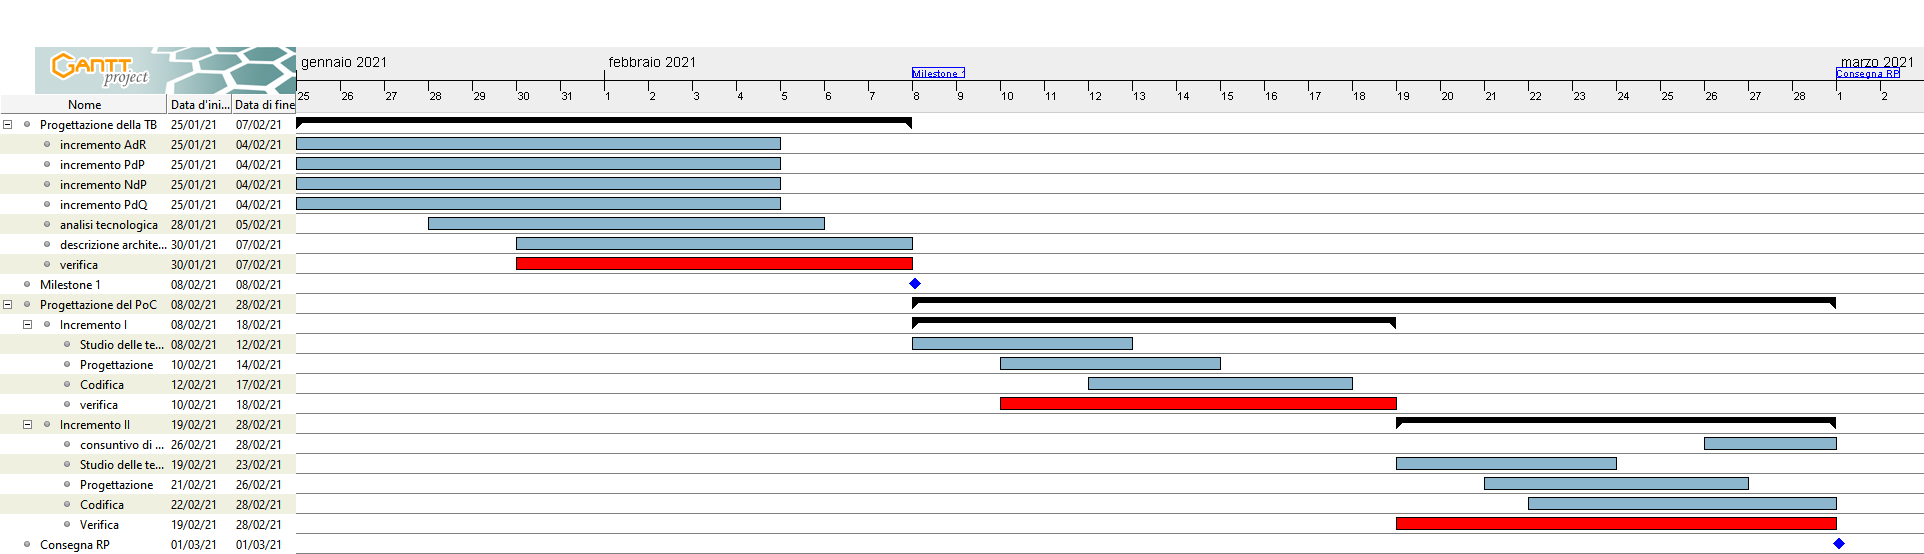
\includegraphics[scale=0.30]{Images/GanttPianificazioneProgettazioneArchitetturale.PNG}
	\caption{Diagramma di Gantt dell'attività di Progettazione Architetturale}
\end{figure}